\documentclass[a4paper]{article}

\usepackage[slovene]{babel}
\usepackage{amsfonts,amssymb,amsmath}
\usepackage[utf8]{inputenc}
\usepackage[T1]{fontenc}
\usepackage{lmodern}
\usepackage{url}

\usepackage{graphicx}

\newtheorem{izrek}{Izrek}
\newtheorem{definicija}{Definicija}
\newtheorem{trditev}{Trditev}
\newtheorem{posledica}{Posledica}
\newtheorem{primer}{Primer}

\def\qed{$\hfill\Box$}   % konec dokaza
\def\qedm{\qquad\Box}   % konec dokaza v matematičnem načinu
\newcommand{\geslo}[2]{\noindent\textbf{#1} \quad \hangindent=1cm #2\\[-1pc]}

\begin{document}

\title{\Huge\textbf{Hiperbolični prostori}} 
\author{\large\textsc{Tjaša Vrhovnik}\\
	Fakulteta za matematiko in fiziko\\
	Oddelek za matematiko}

\thispagestyle{empty}

\maketitle

\newpage

\tableofcontents

\newpage

%%%%%%%%%%%%%%%%%%%%%%%%%%%%%%%%%%%%%%%%%%%%%%%%%%%%%%%%%%%%%%%%%%%%%%%%%%%%
% Uvod
\section{Uvod}

Članek obravnava razred Riemannovih mnogoterosti, imenovanih hiperbolični prostori. Maksimalno simetrične Riemannove mnogoterosti ločimo glede na vrednosti njihove Gaussove ukrivljenosti. Model tistih z ničelno je evklidski prostor $\mathbb{R}^{n}$, $n$-dimenzionalna sfera $\mathbb{S}^{n}(R)$ je modelni prostor s konstantno pozitivno Gaussovo ukrivljenostjo, konstantna negativna Gaussova ukrivljenost pa je lastnost hiperboličnih prostorov $\mathbb{H}^{n}(R)$.

Že samo ime makismalna simetričnost pove, da imajo taki prostori visoko simetrijo. Nekatere lastnosti, ki so posledice tega dejstva, bomo opisali v nadaljevanju. Predstavili bomo štiri osnovne modele $n$-dimenzionalnega hiperboličnega prostora in s konstrukcijo preslikav med njimi dokazali izometričnost modelov. S pomočjo slednjega bomo na vsakem izmed modelov poiskali geodetke ter navedli vrednost Gaussove ukrivljenosti. Čeprav se na prvi pogled zdi, da hiperboličnih prostorov ni mogoče primerjati z evklidskimi, se izkaže, da sta lokalno konformno izomorfna. Na kratko si bomo ogledali hiperbolično geometrijo, ki se je nedolgo nazaj razvila iz ravninske (evklidske) geometrije. 

Študij hiperboličnih prostorov ni zanimiv le z matematične perspektive. Če na $4$-dimenzionalnem hiperboličnem prostoru, natančneje, prostoru Minkowskega, izberemo tri prostorske in eno časovno koordinato, z njim lahko opišemo prostor-čas v teoriji relativnosti. To ima velik pomen za računanje fizikalnih invariant ter nenazadnje razumevanje lastnosti našega vesolja. 

%%%%%%%%%%%%%%%%%%%%%%%%%%%%%%%%%%%%%%%%%%%%%%%%%%%%%%%%%%%%%%%%%%%%%%%%%%%%
% Osnovne definicije
\section{Osnovne definicije}

Naslednje definicije opisujejo mnogoterosti z visoko simetrijo. Natančneje to pomeni, da so njihove grupe izometrij velike. Najpreprostejši primer so Evklidski prostori - zanje že intuitivno vemo, da obstajajo preslikave, izometrije, ki poljubni točki preslikajo eno v drugo, celo več, ortonormirano bazo v prvi točki lahko preslikajo v ortonormirano bazo v drugi. Izkazalo se bo, da to niso edini taki prostori. Drug primer so $n$-dimenzionalne sfere $\mathbb{S}^{n}$, mi pa se bomo posvetili študiju hiperboličnih prostorov.

% izometrija
\begin{definicija}
Naj bosta $(M,g)$ in $(\tilde{M}, \tilde{g})$ Riemannovi mnogoterosti. Gladka preslikava $\phi \colon M \to \tilde{M}$ \emph{ohranja metriko}, če velja $g = \phi^{*}\tilde{g}$.

Difeomorfizem, ki ohranja metriko, imenujemo \emph{izometrija}. \emph{Lokalna izometrija} pa je lokalni difeomorfizem, ki ohranja metriko. 
\end{definicija}

% maksimalna simetričnost
\begin{definicija}
Naj bo $(M,g)$ Riemannova mnogoterost. Množico izometrij mnogoterosti $M$, ki je grupa za komponiranje, označimo z $\textup{Iso}(M,g)$.
Pravimo, da je $(M,g)$ \emph{homogena Riemannova mnogoterost}, če grupa $\textup{Iso}(M,g)$ deluje tranzitivno na $M$. To pomeni, da za poljuben par točk $p,q \in M$ obstaja izometrija $\phi \colon M \to M$ z lastnostjo $\phi(p)=q$.
\end{definicija}

Če je $\phi$ izometrija Riemannove mnogoterosti $(M,g)$, je njen diferencial $d\phi$ preslikava na tangentnem prostoru $TM$. V vsaki točki $p \in M$ diferencial definira linearno izometrijo $d\phi_{p} \colon T_{p}M \to T_{\phi(p)}M$.

\begin{definicija}
Naj bo $p \in M$. Podgrupo grupe $\textup{Iso}(M,g)$ izometrij, ki fiksirajo $p$, imenujemo \emph{izotropična podgrupa} v $p$ in označimo z 
$\textup{Iso}_{p}(M,g)$. 

Preslikavi $I_{p} \colon \textup{Iso}_{p}(M,g) \to \textup{GL}(T_{p}M)$, definirani s predpisom $I_{p}(\phi) = d\phi_{p}$, pravimo \emph{izotropična reprezentacija}.

Mnogoterost $M$ je \emph{izotropična v točki $p$}, kadar izotropična reprezentacija deluje tranzitivno na množico enotskih vektorjev v $T_{p}M$. Nadalje pravimo, da je $M$ \emph{izotropična}, če je izotropična v vsaki točki $p \in M$.
\end{definicija}

Označimo z $\textup{O}(M) = \sqcup_{p \in M} \{ \text{ortonormirane baze} \ T_{p}M \}$ množico vseh ortonormiranih baz na tangentnih prostorih mnogoterosti $M$. Delovanje grupe izometrij $\textup{Iso}(M,g)$ na množico $\textup{O}(M)$ povezuje ortonormirani bazi v točkah $p$ in $\phi(p)$ na naslednji način. Naj bo $\phi \in \textup{Iso}(M,g)$ in $\{e_{1}, \dots , e_{n} \} \in \textup{O}(M)$. Delovanje definiramo s predpisom
\begin{equation}\label{eq:delovanje}
\phi \cdot (e_{1}, \dots , e_{n}) = (d\phi_{p}(e_{1}), \dots , d\phi_{p}(e_{n})).
\end{equation}

\begin{definicija}
Riemannova mnogoterost $(M,g)$ je \emph{maksimalno simetrična}, če je delovanje~\ref{eq:delovanje} tranzitivno na množici $\textup{O}(M)$; natančneje, če za poljuben par $p,q \in M$ in poljuben izbor ortonormiranih baz na tangentnih prostorih $T_{p}M$ in $T_{q}M$ obstaja izometrija, ki preslika $p$ v $q$ ter ortonormirano bazo v točki $p$ v izbrano ortonormirano bazo v točki $q$.
\end{definicija}

Geometrično si homogeno Riemannovo mnogoterost predstavljamo kot tako, ki v vsaki točki na njej izgleda enako.
Izotropična Riemannova mnogoterost pa izgleda enako tudi v vseh smereh.

% konformnost
\begin{definicija}
Naj bosta $(M,g)$ in $(\tilde{M}, \tilde{g})$ Riemannovi mnogoterosti. Difeomorfizem $\phi \colon M \to \tilde{M}$ je \emph{konformna preslikava}, če obstaja taka pozitivna funkcija $\mu \in \mathcal{C}^{\infty}(M)$, da velja
\[ \phi^{*}\tilde{g} = \mu g. \]
V tem primeru pravimo, da sta mnogoterosti $(M,g)$ in $(\tilde{M}, \tilde{g})$ \emph{konformno ekvivalentni}.
\end{definicija}

Konformni difeomorfizmi med Riemannovimi mnogoterostmi so ravno difeomorfizmi, ki ohranjajo velikosti kotov. Tako se pomen zgornje definicije sklada s konformnostjo, ki jo poznamo iz kompleksne analize.

Posebej zanimive Riemannove mnogoterosti so tiste, ki jih (vsaj) lokalno lahko primerjamo z Evklidskim prostorom. Pravimo, da je Riemannova mnogoterost $(M,g)$ \emph{lokalno konformno ploska}, če ima vsaka točka $p\in M$ okolico, ki je konformno ekvivalentna odprti množici v $(\mathbb{R}^{n}, \bar{g})$, kjer $\bar{g}$ označuje običajno Evklidsko metriko. Videli bomo, da imajo hiperbolični prostori to lastnost.

%%%%%%%%%%%%%%%%%%%%%%%%%%%%%%%%%%%%%%%%%%%%%%%%%%%%%%%%%%%%%%%%%%%%%%%%%%%%
% O hiperboličnih prostorih
\section{O hiperboličnih prostorih}
%%%%%%%%%%%%%%%%%%%
% Modeli
\subsection{Modeli}

V tem razdelku bomo navedli modele hiperboličnih prostorov, ki so maksimalno simetrične Riemannove mnogoterosti dimenzije $n \geq 1$. Sprva jih bomo le navedli, kasneje pa pokazali njihovo makismalno simetričnost. Izkaže se, da so vsi ti modeli med seboj izometrični, zato lahko v praksi izberemo kateregakoli izmed njih, na njem obravnavamo želeno in to prenesemo na splošen hiperbolični prostor te dimenzije.

Naj bo $n \geq 1$ in izberimo $R>0$.
\emph{$(n+1)$-dimenzionalni prostor Minkowskega} je prostor $\mathbb{R}^{n,1}$, ki ga v standardnih koordinatah $(x^{1}, \dots , x^{n}, \tau)$ opremimo z \emph{metriko Minkowskega}
\begin{equation}\label{eq:Mink metrika}
\bar{q}^{n,1} = (dx^{1})^2 + \cdots + (dx^{n})^2 - (d\tau)^2.
\end{equation}
Metriko $\bar{q}^{n,1}$ bomo v nadaljevanju označevali preprosto s $\bar{q}$.

\begin{primer}
4-dimenzionalni prostor Minkowskega $\mathbb{R}^{3,1}$ s koordinatami $(x,y,z,t)$ opisuje prostor-čas v Einsteinovi teoriji relativnosti. Grupo izometrij, $\textup{O}(3,1)$, imenovano \emph{Poincar\'ejeva grupa} sestavlja $10$ generatorjev: tri prostorske in ena časovna translacija, tri rotacije (v ravninah $(x,y)$, $(x,z)$, $(y,z)$) in trije Lorentzovi potiski (rotacije v ravninah $(t,x)$, $(t,y)$, $(t,z)$).
\end{primer}

Sedaj definirajmo štiri Riemannove mnogoterosti, ki so osnovni modeli hiperboličnega prostora dimenzije $n$ in polmera $R$.

%%%%%%%%%%%
\begin{enumerate}
\item
% hiperboloid
\textsc{Hiperboloid} $\mathbb{H}^{n}(R)$.

Vzemimo $(n+1)$-dimenzionalni prostor Minkowskega $\mathbb{R}^{n,1}$ s standardnimi koordinatami $(x^{1}, \dots , x^{n}, \tau)$ in metriko $\bar{q}$.
Pozitivni del ($\tau > 0$) dvodelnega hiperboloida $(x^{1})^2 + \cdots + (x^{n})^2 - \tau^2 = -R^2$ opremimo z metriko
\begin{equation}\label{eq:H^n metrika}
\u g_{R}^{1} = \iota^{*}\bar{q},
\end{equation}
kjer $\iota$ označuje inkluzijo $\iota \colon \mathbb{H}^{n}(R) \to \mathbb{R}^{n,1}$. Dobljeno podmnogoterost $(\mathbb{H}^{n}(R), \u g_{R}^{1})$ imenujemo \emph{hiperboloid} dimenzije $n$ s polmerom $R$.

\item
% Beltrami-Klein
\textsc{Beltrami-Kleinov model} $\mathbb{K}^{n}(R)$

Na $n$-dimenzionalni krogli $\mathbb{K}^{n}(R)$ s središčem v izhodišču prostora $\mathbb{R}^{n}$ in polmerom $R$ uvedimo koordinate $(w^{1}, \dots , w^{n})$. Kroglo opremimo z metriko
\begin{equation}\label{eq:K^n metrika}
\u g_{R}^{2} = R^2 \frac{(dw^{1})^2 + \cdots + (dw^{n})^2}{R^2-|w|^2} + R^2 \frac{(w^{1}dw^{1} + \cdots + w^{n}dw^{n})^2}{(R^2-|w|^2)^2}.
\end{equation}
Mnogoterost $(\mathbb{K}^{n}(R), \u g_{R}^{2})$ se imenuje \emph{Beltrami-Kleinov model}.

\item
% Poincarejeva korgla
\textsc{Poincar\'ejeva krogla} $\mathbb{B}^{n}(R)$

Na $n$-dimenzionalni krogli $\mathbb{B}^{n}(R)$ s središčem v izhodišču prostora $\mathbb{R}^{n}$ in polmerom $R$ uvedimo koordinate $(u^{1}, \dots , u^{n})$. Kroglo opremimo z metriko
\begin{equation}\label{eq:K^n metrika}
\u g_{R}^{3} = 4R^4 \frac{(du^{1})^2 + \cdots + (du^{n})^2}{(R^2-|u|^2)^2}.
\end{equation}
Mnogoterost $(\mathbb{B}^{n}(R), \u g_{R}^{3})$ definira \emph{Poincar\'ejevo kroglo}.

\item
% Poincarejev polprostor
\textsc{Poincar\'ejev polprostor} $\mathbb{U}^{n}(R)$

Na Evklidskem prostoru $\mathbb{R}^{n}$ uvedimo koordinate $(x^{1}, \dots , x^{n-1}, y)$ in njegov podprostor $\mathbb{U}^{n}(R) = \{ (x,y); \ y>0 \}$ opremimo z metriko
\begin{equation}\label{eq:K^n metrika}
\u g_{R}^{4} = R^2 \frac{(dx^{1})^2 + \cdots + (dx^{n-1})^2 + dy^2}{y^2}.
\end{equation}
Mnogoterosti $(\mathbb{U}^{n}(R), \u g_{R}^{4})$ pravimo \emph{Poincar\'ejev polprostor}.
%
\end{enumerate}
%%%%%%%%%%

Zaradi izometričnosti zgornjih modelov pogosto hiperbolični prostor dimenzije $n$ s polmerom $R$ označimo z $\mathbb{H}^{n}(R)$, metriko pa z $\u g_{R}$, pri čemer imamo v mislih poljubnega izmed modelov. Če za polmer izberemo $R=1$, Riemannovo mnogoterost označimo s $(\mathbb{H}^{n}, \u g)$ in imenujemo \emph{hiperbolični prostor} dimenzije $n$. V dveh dimenzijah dobimo \emph{hiperbolično ravnino}, h kateri se bomo vrnili kasneje.

% Primer - Poincar\'ejeva krogla
\begin{primer}
Vzemimo enotsko $n$-dimenzionalno Poincar\'ejevo kroglo $\mathbb{B}^{n}(1)$. Izračunajmo razdaljo med izhodiščem in točko $P = (R,0, \dots , 0)$ v Poincar\'ejevi krogli:
\begin{gather}
r = d(0, P) = \int_{0}^{R} \sqrt{\u g_{1}^{3}} = \int_{0}^{R} \frac{2ds}{1-|s|^2} = \ln{\frac{1+R}{1-R}}.
\end{gather}
Ko se točka $P$ približuje robu krogle, njena hiperbolična razdalja do izhodišča raste v neskončnost.
S preoblikovanjem zgornje zveze dobimo 
\begin{gather}
R = \frac{e^{r}-1}{e^{r}+1} = \tanh{\frac{r}{2}},
\end{gather}
ki pove, kako se (evklidski) polmer Poincar\'ejeve krogle $\mathbb{B}^{n}(R)$ izraža s hiperbolično razdaljo $r$.\newline 
Kolikšna pa je njena prostornina?
Naj bo $d\mu^{n}(w)$ volumski element za $\mathbb{B}^{n}(R)$ (koordinate $w=(u,v)$). Velja $d\mu^{n}(w) = u^{n-1} d\textup{Vol}(\mathbb{S}^{n-1})(v)$. Sledi 
\begin{align*}
\textup{Vol}(\mathbb{B}^{n}(R)) &= \int_{\mathbb{B}^{n}(R)} \frac{2^{n} d\mu^{n}(s)}{(1-|s|^2)^{n}} = \textup{Vol}(\mathbb{S}^{n-1}) \int_{0}^{R} \frac{2^{n} y^{n-1}}{(1-y^{2})^{n}} dy \\ 
&= 2^{n-1} \textup{Vol}(\mathbb{S}^{n-1}) \int_{0}^{\tanh{\frac{r}{2}}} \frac{2 y^{n-1}}{(1-y^{2})^{n}} dy \quad \left[y = \tanh{\frac{x}{2}} \right] \\
&= 2^{n-1} \textup{Vol}(\mathbb{S}^{n-1}) \int_{0}^{r} \sinh^{n-1}{\frac{x}{2}} \cosh^{n-1}{\frac{x}{2}} dx \\
&= \textup{Vol}(\mathbb{S}^{n-1}) \int_{0}^{r} \sinh^{n-1}{x} dx
\end{align*}
Opazimo, da za velike $r$, tj.~v limiti, ko gre $r \to \infty$, dobimo približno oceno
\begin{gather*}
\textup{Vol}(\mathbb{B}^{n}(R)) \sim \frac{1}{2^{n-1}} \textup{Vol}(\mathbb{S}^{n-1}) e^{r(n-1)}.
\end{gather*}
Z besedami to pomeni, da je prostornina Poincar\'ejeve krogle eksponentno odvisna od njenega polmera. V Evklidskih prostorih je odvisnost polinomska.
\end{primer}

%%%%%%%%%%%%%%%%%%%
% Izometričnost modelov
\subsection{Izometričnost modelov}

\begin{izrek}
Modeli $n$-dimenzionalnih hiperboličnih prostorov s polmerom $R$ so paroma izometrični.
\end{izrek}

Dokaz bo potekal v več korakih. Najprej bomo preverili, da je hiperbolični prostor Riemannova mnogoterost. Nato bomo konstruirali izometrije med naslednjimi pari modelov: hiperboloidom in Beltrami-Kleinovim modelom, hiperboloidom in Poincar\'ejevo kroglo ter Poincar\'ejevim polprostorom in Poincar\'ejevo kroglo.

Dokažimo najprej, da je hiperboloid $\mathbb{H}^{n}(R)$ Riemannova podmnogoterost prostora $\mathbb{R}^{n,1}$. To zadostuje, saj bo iz izometričnosti sledilo, da so vsi modeli Riemannove mnogoterosti.
Prostor $\mathbb{H}^{n}(R)$ lahko opišemo kot 
\begin{equation}\label{eq:H^n enacba}
\mathbb{H}^{n}(R) = F^{-1}(-R^2) \cap \{ \tau>0 \},
\end{equation}
kjer je preslikava $F \colon \mathbb{R}^{n+1} \to \mathbb{R}$ definirana s predpisom $F(x^{1}, \dots , x^{n}, \tau) = \sum_{i=1}^{n} (x^{i})^2 - \tau^2$.
Tangentni prostor v točki $p \in \mathbb{H}^{n}(R)$, ki je enak $T_{p}\mathbb{H}^{n}(R) = \ker dF_{p}$, razpenjajo vektorji $X^{i} = \tau \frac{\partial}{\partial x^{i}} + x^{i} \frac{\partial}{\partial \tau}$ za $i = 1, \dots , n$. Ker je njihov produkt (glede na metriko $\bar{q}$) pozitiven, je metrika $\u g_{R}^{1}$ pozitivno definitna in določa Riemannovo podmnogoterost $(\mathbb{H}^{n}(R), \u g_{R}^{1})$. 

% Centralna projekcija
\subsubsection{Centralna projekcija}
Izometrija med hiperboloidom in Beltrami-Kleinovim modelom se imenuje \emph{centralna projekcija}, $c \colon \mathbb{H}^{n}(R) \to \mathbb{K}^{n}(R)$.

Naj bo $T=(x^{1}, \dots , x^{n}, \tau) \in \mathbb{H}^{n}(R)$ poljubna točka. Presečišče premice $OT$ skozi izhodišče v $\mathbb{R}^{n,1}$ in točko $T$ s hiperravnino $\{ (x, \tau); \ \tau=R \}$ označimo z $Y \in \mathbb{R}^{n,1}$. Pišimo $Y=(y,R)$, kjer je $y = c(T) \in \mathbb{K}^{n}(R)$ slika $T$ s centralno projekcijo. 
Tedaj se koordinate točke $Y$ izražajo s koordinatami $T$, natančneje, $Y=\frac{R}{\tau} T$. Preslikavo $c$ zato podaja zveza
\begin{equation}\label{eq: cent-proj}
c(x, \tau) = \frac{R}{\tau} x.
\end{equation}
Ker slika točke s preslikavo $c$ leži na hiperboloidu, velja
\[ |c(x,\tau)|^2 = \frac{R^2}{\tau^2} |x|^2 = \frac{R^2}{\tau^2}(\tau^2-R^2) = R^2 \left(1-\frac{R^2}{\tau^2} \right) < R^2, \]
torej je $c(x, \tau) \in \mathbb{K}^{n}(R)$ in je centralna projekcija dobro definirana.

Da je preslikava $c$ difeomorfizem, bomo pokazali s konstrukcijo njenega inverza.
Vzemimo poljubno točko $y \in \mathbb{K}^{n}(R)$. Potem obstaja enoličen $\lambda>0$, da velja $(x, \tau) = \lambda (y,R) \in \mathbb{H}^{n}(R)$. Slednja točka je določena z zvezo $\lambda^2 (|y|^2-R^2)=-R^2$, od koder sledi $\lambda = \frac{R}{(R^2-|y|^2)^{1/2}}$.
Potem predpis
\begin{equation}\label{eq:c^{-1}}
c^{-1}(y) = \left( \frac{Ry}{(R^2-|y|^2)^{1/2}}, \frac{R^2}{(R^2-|y|^2)^{1/2}} \right)
\end{equation}
definira gladko preslikavo, ki je inverz centralne projekcije.

Nazadnje dokažimo, da je $c$ izometrija. Želimo videti, da velja enakost $(c^{-1})^{*} \u g_{R}^{1} = \u g_{R}^{2}$.
Diferenciali točke $(x, \tau) = c^{-1}(y)$ iz enačbe~\ref{eq:c^{-1}} za nek $y \in \mathbb{K}^{n}(R)$ so enaki
\begin{gather*}
dx^{i} = \frac{Rdy^{i}}{(R^2-|y|^2)^{1/2}} + \frac{Ry^{i} \sum_{k=1}^{n}y^{k}dy^{k}}{(R^2-|y|^2)^{3/2}}, \\
d\tau = \frac{R^2 \sum_{k=1}^{n}y^{k}dy^{k}}{(R^2-|y|^2)^{3/2}}.
\end{gather*}
Od tod izračunamo
\[ (c^{-1})^{*} \u g_{R}^{1} = \sum_{i=1}^{n} (dx^{i})^2 - (d\tau)^2 = R^2 \frac{\sum_{i=1}^{n}(dy^{i})^2}{R^2-|y|^2} + R^2 \frac{(\sum_{i=1}^{n}y^{i}dy^{i})^2}{(R^2-|y|^2)^2} = \u g_{R}^{2}. \]
Torej je centralna projekcija res izometrija med $(\mathbb{H}^{n}(R), \u g_{R}^{1})$ in $(\mathbb{K}^{n}(R), \u g_{R}^{2})$.

% Hiperbolična stereografska projekcija
\subsubsection{Hiperbolična stereografska projekcija}
Izometriji med hiperboloidom in Poincar\'ejevo kroglo pravimo \emph{hiperbolična stereografska projekcija}, $h \colon \mathbb{H}^{n}(R) \to \mathbb{B}^{n}(R)$. Spominja na običajno stereografsko projekcijo za sfere, zato je tudi njena konstrukcija podobna le-tej.

Naj bo $S=(0, \dots , -R) \in \mathbb{R}^{n,1}$ in izberimo poljubno točko $T=(x^{1}, \dots , x^{n}, \tau)$ na hiperboloidu. Označimo presečišče premice $ST$ s hiperravnino $\{ (x, \tau); \ \tau=0 \}$ z $V=(v,0) \in \mathbb{R}^{n,1}$ in postavimo $h(T)=v \in \mathbb{B}^{n}(R)$.
Sedaj bomo izračunali predpis, ki definira preslikavo $h$.
Po konstrukciji točke $V$ obstaja enoličen $\lambda>0$, ki zadošča enakosti $V-S=\lambda(T-S)$. Ekvivalentno lahko po komponentah zapišemo
\begin{align*}
v^{i} &= \lambda x^{i}, \quad  i=1, \dots n, & R &= \lambda(\tau+R),
\end{align*}
od koder izračunamo koeficient $\lambda = \frac{R}{\tau+R}$. Formula, ki določa $h$, je enaka
\begin{equation}\label{eq: hip-ster-proj}
h(x,\tau) = \frac{R}{\tau+R}x.
\end{equation}
Ker točka $(x,\tau)$ leži na hiperboloidu, ocenimo
\[ |h(x,\tau)|^2 = \frac{R^2}{(\tau+R)^2} |x|^2 = R^2 \frac{\tau^2-R^2}{\tau^2+R^2} < R^2, \]
zato preslikava $h$ res slika v Poincar\'ejevo kroglo $\mathbb{B}^{n}(R)$.

Konstruirajmo inverz preslikave. Komponente točke $T \in \mathbb{H}^{n}(R)$ se v odvisnosti od koeficienta $\lambda$ izražajo kot
\begin{align*}
x^{i} &= \frac{v^{i}}{\lambda}, \quad  i=1, \dots n, & \tau &= R \frac{1-\lambda}{\lambda}.
\end{align*}
To vstavimo v pogoj za točko na hiperboloidu, $|x|^2-\tau^2=-R^2$, kar nam da $\lambda = \frac{R^2-|v|^2}{2R^2}$.
Inverzna preslikava ima potem predpis
\begin{equation}\label{eq:h^{-1}}
h^{-1}(v) = \left( \frac{2R^2v}{R^2-|v|^2}, R \frac{R^2+|v|^2}{R^2-|v|^2} \right).
\end{equation} 
Gladek inverz nam zagotavlja, da je hiperbolična stereografska projekcija difeomorfizem.

Podobno kot v prejšnjem primeru preverimo še enakost $(h^{-1})^{*} \u g_{R}^{1} = \u g_{R}^{3}$.
Diferenciali komponent točke $(x,\tau)=h^{-1}(v)$ iz predpisa~\ref{eq:h^{-1}} so
\begin{gather*}
dx^{i} = \frac{2R^2dv^{i}}{R^2-|v|^2} + \frac{4R^2v^{i} \sum_{k=1}^{n}v^{k}dv^{k}}{(R^2-|v|^2)^2}, \\
d\tau = \frac{2R \sum_{k=1}^{n}v^{k}dv^{k}}{R^2-|v|^2} + \frac{2R(R^2+|v|^2) \sum_{k=1}^{n}v^{k}dv^{k}}{(R^2-|v|^2)^2}.
\end{gather*}
Z nekaj računanja dobimo
\[ (h^{-1})^{*} \u g_{R}^{1} = \sum_{i=1}^{n} (dx^{i})^2 - (d\tau)^2 = \u g_{R}^{3}. \]
Pokazali smo, da je hiperbolična stereografska projekcija izometrija prostorov $(\mathbb{H}^{n}(R), \u g_{R}^{1})$ in $(\mathbb{B}^{n}(R), \u g_{R}^{3})$.

% Cayleyjeva transformacija
\subsubsection{Posplošena Cayleyjeva transformacija}
Omenimo še konstrukcijo izometrije med Poincar\'ejevo polravnino in Poincar\'ejevo kroglo. 
V dvodimenzionalnem primeru smo v domači nalogi videli, da izometrijo med Poincar\'ejevo polravnino $\mathbb{U}$ in Poincar\'ejevim diskom $\mathbb{D}$ (za $R=1$) podaja M\"obiusova transformacija $\tau \colon \mathbb{U} \to \mathbb{D}$, definirana s predpisom
\begin{equation}
\tau(z) = \frac{1+iz}{z+i},
\end{equation} 
kjer je $z=(x,y)$ kompleksen zapis točke v ravnini. S skaliranjem dobimo predpis za preslikavo $k \colon \mathbb{U}^{2}(R) \to \mathbb{B}^{2}(R)$,
\begin{equation}
k(z) = iR \frac{z-iR}{z+iR}.
\end{equation} 
Če preidemo v realne koordinate z identifikacijo $\Re{z}=x$, $\Im{z}=y$, kratek račun pokaže ekvivalenten predpis
\begin{equation}
k(x,y) = \left( \frac{2xR^2}{x^2+(y+R)^2}, R \frac{x^2+y^2-R^2}{x^2+(y+R)^2} \right).
\end{equation}
Preslikavi $k$ pravimo \emph{Cayleyjeva transformacija}.

V splošnem primeru koordinate na Poincar\'ejevem polprostoru $\mathbb{U}^{n}(R)$ zapišimo kot $(x^{1}, \dots , x^{n}, y) = (x,y)$ in uporabimo zgornji predpis. Novo preslikavo, ki je prav tako izometrija, imenujemo \emph{posplošena Cayleyjeva transformacija}.

%%%%%%%%%%%%%%%%%%%
% Lastnosti hiperboličnih prostorov
\subsection{Lastnosti hiperboličnih prostorov}

\begin{trditev}
Hiperbolični prostor $(\mathbb{H}^{n}(R), \u g)$ je lokalno konformno ploščat.
\end{trditev}

\noindent
{\em Dokaz:\/} 
Za model hiperboličnega prostora vzemimo Poincar\'ejevo kroglo  $\mathbb{B}^{n}(R)$. Identična preslikava $id \colon (\mathbb{B}^{n}(R), \u g_{R}^{3}) \to (\mathbb{R}^{n}, \bar{g})$ je konformna in porodi konformno ekvivalenco Poincar\'ejeve krogle z odprto podmnožico Evklidskega prostora. Zaradi izometričnosti modelov sledi, da je hiperbolični prostor lokalno konformno ploščat.
\qed

% Lorentzova grupa
\begin{definicija}
Naj bo $\mathbb{R}^{n,1}$ prostor Minkowskega ($n \geq 1$) opremljen z metriko Minkowskega $\bar{q}$. Grupo linearnih preslikav, ki slikajo $\mathbb{R}^{n,1}$ vase in ohranjajo metriko Minkowskega, imenujemo \emph{($n+1$)-dimenzionalna Lorentzova grupa} in označimo z $\textup{O}(n,1)$.

Njeno podgrupo, ki ohranja hiperboloid $\mathbb{H}^{n}(R)$ označimo z $\textup{O}^{+}(n,1)$. Pravimo ji \emph{ortokrona Lorentzova grupa}.
\end{definicija}

\begin{trditev} \label{trd: frame-homo}
Lorentzova grupa $\textup{O}^{+}(n,1)$ deluje tranzitivno na množico $\textup{O}(\mathbb{H}^{n}(R))$. Hiperbolični prostor $\mathbb{H}^{n}(R)$ je makismalno simetričen.
\end{trditev}

\noindent
{\em Dokaz:\/} 
Dovolj je pokazati, da za poljubno točko $p \in \mathbb{H}^{n}(R)$ in ortonormirano bazo $\{e_{1}, \dots , e_{n} \}$ prostora $T_{p}\mathbb{H}^{n}(R)$ obstaja ortogonalna preslikava, ki preslika točko $N=(0, \dots , 0, R)$ v $p$ ter ortonormirano bazo $\{\partial_{1}, \dots , \partial_{n} \}$ za $T_{N}\mathbb{H}^{n}(R)$ v bazo $\{e_{i}\}_{i}$.

Naj bo $p \in \mathbb{H}^{n}(R)$ poljubna točka. Identificirajmo $p$ z vektorjem dolžine $R$ v $T_{p}\mathbb{R}^{n,1}$  in postavimo $\bar{p} = \frac{p}{R}$. $\bar{p}$ je enotski vektor glede na metriko Minkowskega $\bar{q}$, kaže v smeri $p$, in $\bar{p} \in T_{p}\mathbb{R}^{n,1}$.
Prostor $\mathbb{H}^{n}(R)$ predstavimo kot v~\ref{eq:H^n enacba}.
Tedaj je gradient preslikave $F$ glede na metriko $\bar{q}$ enak
\begin{equation}
\textup{grad} F = 2 \sum_{i=1}^{n} x^{i} \frac{\partial}{\partial x^{i}} + 2\tau \frac{\partial}{\partial \tau}. \nonumber
\end{equation} 
Opazimo, da je $\bar{p} = 2 \cdot \textup{grad} F$ in zato $\bar{p} \perp T_{p}\mathbb{H}^{n}(R)$.
Potem je množica $\{ e_{1}, \dots , e_{n}, \bar{p} \}$ ortonormirana baza prostora $\mathbb{R}^{n,1}$ glede na metriko $\bar{q}$.

Naj bo $M$ matrika, katere stolpci so vektorji iz zgornje ortonormirane baze. Po konstrukciji velja $M \in \textup{O}^{+}(n,1)$ in $M$ slika $\{\partial_{1}, \dots , \partial_{n+1} \}$ v $\{e_{1}, \dots , e_{n}, \bar{p} \}$ ter $N$ v $p$.
Ker je $M$ kot preslikava linearna na $\mathbb{R}^{n,1}$, je njen diferencial v točki $N$, $dM_{N} \colon T_{N}\mathbb{R}^{n,1} \to T_{p}\mathbb{R}^{n,1}$, prav tako predstavljen z matriko $M$. To pa pomeni, da je $dM_{n}(\partial_{i}) = e_{i}$, $i = 1, \dots , n$.
$M$ je iskana preslikava in delovanje grupe je tranzitivno. Po definiciji je zato $\mathbb{H}^{n}(R)$ maksimalno simetričen.
\qed
\newline

% simetričnost
Lastnost hiperboličnih prostorov, ki jo bomo dokazali v nadaljevanju, je šibkejša od maksimalne simetričnosti, a močnejša od homogenosti. Sprva jo definirajmo.

\begin{definicija}
Naj bo $(M,g)$ Riemannova mnogoterost in $p\in M$ točka na njej. Izometriji $\phi \colon M \to M$, za katero velja $\phi(p) = p$ in $d\phi_{p} = -\textup{Id} \colon T_{p}M \to T_{p}M$, pravimo \emph{točkovno zrcaljenje} v točki $p$.

Povezana Riemannova mnogoterost $(M,g)$ je \emph{simetrična}, če v vsaki točki $p \in M$ premore točkovno zrcaljenje v $p$.
\end{definicija}

\begin{trditev}
Hiperbolični prostor je simetričen.
\end{trditev}

\noindent
{\em Dokaz:\/} 
Naj bo $(M,g)$ povezana maksimalno simetrična Riemannova mnogoterost. Naj bo $p \in M$ poljubna točka in izberimo ortonormirano bazo $\{ e_{i} \}_{i}$ za $T_{p}M$. Ker je mnogoterost maksimalno simetrična, obstaja izometrija $\phi \colon M \to M$, ki $p$ preslika vase, ortonormirano bazo $\{e_{i} \}_{i}$ pa preslika v $\{ -e_{i} \}_{i}$. Torej zadošča $d\phi_{p} = -\textup{Id}$. To pa je natanko simetričnost.

V posebnem, hiperbolični prostor je povezana Riemannova mnogoterost in po že dokazanem maksimalno simetričen. Iz zgornjega sledi njegova simetričnost. 
\qed

%%%%%%%%%%%%%%%%%%%
% Ukrivljenost
\subsection{Ukrivljenost}

Gaussova ukrivljenost $\kappa$ ploskve v točki je po definiciji enaka produktu glavnih ukrivljenosti v tej točki. 
Ničelna Gaussova ukrivljenost karakterizira ploskve, ki so lokalno izomorfne ravnini.
Ploskve s pozitivno Gaussovo ukrivljenostjo v točki imajo lastnost, da sta glavni ukrivljenosti v točki istega predznaka (odvisni od izbora normale). Primer take ploskve je 2-sfera $\mathbb{S}^{2}(R)$ polmera $R$, za katero velja $\kappa = 1/R^2$. 
Negativna Gaussova ukrivljenost pa pomeni, da vektorja glavnih ukrivljenosti kažeta v nasprotno smer. Geometrijsko ima ploskev v taki točki obliko sedla. 

Za študij so posebej zanimive ploskve s konstantno Gaussovo ukrivljenostjo. Najprej si oglejmo primer.

% Primer - traktoid
\begin{primer}[Traktoid]
Opazujmo ploskev, vloženo v $\mathbb{R}^{3}$, in izračunajmo njeno Gaussovo ukrivljenost.
Defnirajmo preslikavi
\begin{align*}
f &\colon (0,1) \to \mathbb{R}, &f(r) &= \sqrt{1-r^2} - \cosh ^{-1} \left(\frac{1}{r} \right); \\
\sigma &\colon (0,1) \times (0,2\pi) \to \mathbb{R}^{3}, &\sigma(r,v) &= (r \cos{v}, r \sin{v}, f(r)).
\end{align*}
Preslikava $\sigma$ je parametrizacija rotacijske ploskve, ki jo imenujemo \emph{traktoid}.

Izračunajmo prvo in drugo fundamentalno formo ploskve.
\begin{gather*}
\sigma_{r} = \left(\cos{v}, \sin{v}, \frac{\sqrt{1-r^2}}{r} \right), \  \sigma_{v} = \left(-r \sin{v}, r \cos{v}, 0 \right), \\
\sigma_{rr} = \left(0, 0, -\frac{1}{r^2 \sqrt{1-r^2}} \right), \  \sigma_{rv} = \sigma_{vr} = (-\sin{v}, \cos{v}, 0), \  \sigma_{vv} = (-r\cos{v}, -r\sin{v}, 0), \\
\sigma_{r} \times \sigma_{v} = \left(-\sqrt{1-r^2}\cos{v}, -\sqrt{1-r^2}\sin{v}, r \right), \  ||\sigma_{r} \times \sigma_{v}|| = 1, \\
n = -\frac{\sigma_{r} \times \sigma_{v}}{||\sigma_{r} \times \sigma_{v}||} = \left(\sqrt{1-r^2}\cos{v}, \sqrt{1-r^2}\sin{v}, -r \right),
\end{gather*}
kjer je $n$ zunanja normala ploskve. Iz parcialnih odvodov izračunamo koeficiente
\begin{gather*}
E = \sigma_{r} \cdot \sigma_{r} = \frac{1}{r^2}, \ F = \sigma_{r} \cdot \sigma_{v} = 0, \ G = \sigma_{v} \cdot \sigma_{v} = r^2, \\
L = \sigma_{rr} \cdot n = \frac{1}{r\sqrt{1-r^2}}, \ M = \sigma_{rv} \cdot n = 0, \ N = \sigma_{vv} \cdot n = -r\sqrt{1-r^2}.
\end{gather*}
Po formuli za Gaussovo ukrivljenost končno dobimo
\begin{gather*}
\kappa = \frac{LN-M^2}{EG-F^2} = -1.
\end{gather*}
\end{primer}
%
\begin{figure}[h!]
\begin{center}
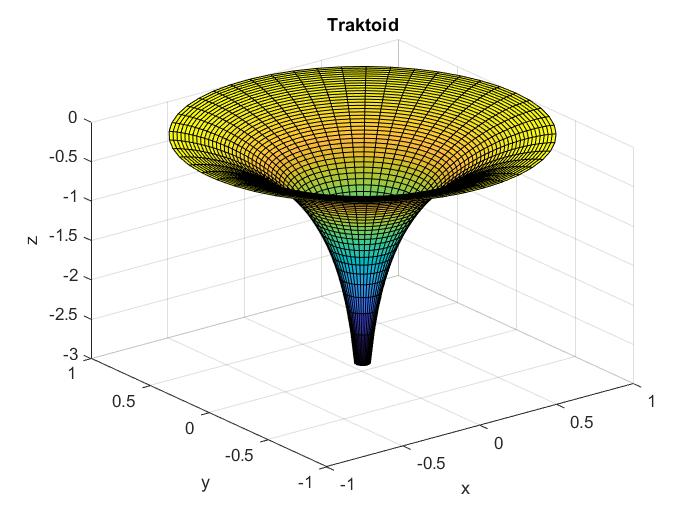
\includegraphics[scale=0.35]{traktoid.jpg}
\caption{Traktoid s $\kappa = -1$.}
\end{center}
\end{figure}
%
Traktoid ima konstantno negativno Gaussovo ukrivljenost in spada med hiperbolične ploskve. S ploskev, tj.~dvodimenzionalnih prostorov, lahko preidemo na prostore poljubnih dimenzij. V razredu smo izračunali Gaussovo ukrivljenost hiperboloida $\mathbb{H}^{n}(R)$, ki je enaka 
\begin{gather}
\kappa (\mathbb{H}^{n}(R)) = \left(-\frac{1}{iR} \right)^n.
\end{gather}
 Za fiksen izbor števil $n \in \mathbb{N}, \ R>0$ je $\kappa = \mbox{konst.}<0$. Ker je $\mathbb{H}^{n}(R)$ model hiperboličnega prostora dimenzije $n$ in polmera $R$, ter so vsi modeli med seboj izometrični, ima vsak hiperbolični prostor konstantno negativno Gaussovo ukrivljenost. Velja tudi $\textup{sec}(\mathbb{H}^{n}(R)) = -1/R^2$, kjer $\textup{sec}$ označuje \emph{prerezno ukrivljenost}. Za poljubne $R>0$ dobimo vse možne vrednosti konstantno negativne prerezne ukrivljenosti, ki ustrezajo hiperboličnim prostorom polmera $R$.

Naslednji rezultat bomo le navedli brez dokaza. Povzet je po \cite[Theorem 12.4 (Killing-Hopf)]{leeRM}. Pomemben in zanimiv je zato, ker klasificira Riemannove mnogoterosti glede na njihovo prerezno ukrivljenost.

\begin{izrek}[Killing-Hopf]
Naj bo $n \geq 2$ in $(M,g)$ polna~\footnote{Riemannova mnogoterost je \emph{polna}, če so maksimalne geodetke definirane za vse $t \in \mathbb{R}$.} enostavno povezana~\footnote{Spomnimo se, da je s potmi povezana topološka mnogoterost \emph{enostavno povezana} natanko tedaj, ko ima trivialno prvo fundamentalno grupo.} 
Riemannova mnogoterost dimenzije $n$ s konstantno prerezno ukrivljenostjo. Potem je $M$ izometrična natanko enemu izmed prostorov: Evklidskemu prostoru $\mathbb{R}^{n}$, $n$-sferi $\mathbb{S}^{n}(R)$ ali hiperboličnemu prostoru $\mathbb{H}^{n}(R)$.
\end{izrek}

Ker po zgornjih ugotovitvah vemo, da imajo hiperbolični prostori konstantno negativno prerezno ukrivljenost, bi model hiperboličnega prostora lahko definirali kot polno enostavno povezano Riemannovo mnogoterost s konstantno negativno prerezno ukrivljenostjo.

%%%%%%%%%%%%%%%%%%%
% Geodetke na hiperboličnih prostorih
\subsection{Geodetke na modelih hiperboličnih prostorov}

\begin{izrek}
Maksimalne geodetke na hiperboličnem prostoru so natanko
\begin{enumerate}
\item glavne hiperbole, natančneje, preseki $\mathbb{H}^{n}(R)$ z ravnino v $\mathbb{R}^{n,1}$, če je prostor \textup{hiperboloid} $\mathbb{H}^{n}(R)$;
%
\item premice v notranjosti $\mathbb{K}^{n}(R)$ v \textup{Beltrami-Kleinovem modelu} $\mathbb{K}^{n}(R)$;
%
\item premeri krogle $\mathbb{B}^{n}(R)$ ali krožni loki v notranjosti krogle, ki rob $\partial\mathbb{B}^{n}(R)$ sekajo pod pravim kotom, v primeru \textup{Poincar\'ejeve krogle} $\mathbb{B}^{n}(R)$;
%
\item premice, vzporedne $\tau$-osi, ali polkrožnice s središči na robu $\partial\mathbb{U}^{n}(R)$, kadar je model \textup{Poincar\'ejev polprostor} $\mathbb{U}^{n}(R)$.
\end{enumerate}
Dodatno, hiperbolični prostor je geodetsko poln (maksimalne geodetke obstajajo za vse $t \in \mathbb{R}$).
\end{izrek}

% dokaz geodetk
\noindent
{\em Dokaz:\/}
% hiperboloid
Najprej bomo obravnavali model hiperboloida $\mathbb{H}^{n}(R)$.
Opazimo, da je na hiperboloidu tangentna komponenta povezave $\nabla^{\perp}$ enaka Levi-Civita, saj je $\mathbb{H}^{n}(R)$ vložena podmnogoterost v $\mathbb{R}^{n,1}$.
Geodetke na hiperboloidu zato lahko karakteriziramo z naslednjim pogojem: krivulja $\gamma \colon I \subset \mathbb{R} \to \mathbb{H}^{n}(R)$ je geodetka natanko tedaj, ko je za vse $t$ vektor $\gamma''(t)$ pravokoten na tangentni prostor $T_{\gamma(t)}\mathbb{H}^{n}(R)$ glede na metriko Minkowskega $\bar{q}$.

Vzemimo poljubno točko $p \in \mathbb{H}^{n}(R)$ in jo kot v dokazu trditve~\ref{trd: frame-homo} identificirajmo z vektorjem dolžine $R$ v $T_{p}\mathbb{R}^{n,1}$. Naj bo $F$ funkcija, ki definira hiperboloid (enakost~\ref{eq:H^n enacba}).
Opisati želimo elemente tangentnega prostora $T_{p}\mathbb{H}^{n}(R)$. Ker velja $\textup{grad}F|_{p}=2\cdot p$, neničelni vektor $v$ zadošča $v \in T_{p}\mathbb{H}^{n}(R)$ natanko takrat, ko je $\bar{q}(p,v)=0$ (vektorja $p$ in $v$ sta pravokotna glede na metriko $\bar{q}$).

Izberimo $v \in T_{p}\mathbb{H}^{n}(R)$ ter postavimo $a=\frac{|v|_{\bar{q}}}{R}$ in $\bar{v}=\frac{v}{a}$ (tj.~$|\bar{v}|=R$).
Definirajmo gladko krivuljo $\gamma \colon \mathbb{R} \to \mathbb{R}^{n,1}$ s predpisom
\[ \gamma(t) = \cosh(at) \cdot p + \sinh(at) \cdot \bar{v}. \]
Krivulja leži na hiperboloidu, saj velja $ |\sinh(at) \cdot \bar{v}|^2 - |\cosh(at) \cdot p|^2 = -R^2$. Nadalje je 
\begin{gather*}
\gamma'(t) = a\sinh(at) \cdot p + a\cosh(at) \cdot \bar{v}, \\
\gamma''(t) = a^2\cosh(at) \cdot p + a^2\sinh(at) \cdot \bar{v} = a^2 \gamma(t), \\
\bar{q}(\gamma'(t), \gamma''(t)) = 0,
\end{gather*}
od koder sledi, da je krivulja $\gamma$ geodetka v $\mathbb{H}^{n}(R)$.
Veljata še začetna pogoja $\gamma(0)=p$ in $\gamma'(0)=a\bar{v}=v$, zato je $\gamma = \gamma_{v}$ konstantne hitrosti $a$.
Krivulja $\gamma_{v}$ je gladka vložitev $\mathbb{R} \to \mathbb{H}^{n}(R)$, katere slika je glavna hiperbola (ravnino, ki seka hiperboloid, razpenjata vektorja $p, \ \bar{v}$).

Naj bo $\Sigma \subset \mathbb{R}^{n,1}$ taka ravnina z ortonormirano bazo $\{v,p\}$, da je njen presek s hiperboloidom $\mathbb{H}^{n}(R)$ glavna hiperbola $H$. Potem je $H$ slika geodetke z začetno točko $p$ (točka $p$ in pripadajoč vektor sta identificirana) in začetno hitrostjo $v$.\newline

Dokazali smo, da so maksimalne geodetke na hiperboloidu natanko glavne hiperbole. Modeli hiperboličnih prostorov so med seboj izometrični, zato zaradi naravnosti Levi-Civita sledi, da so geodetke v vseh modelih vložitve $\mathbb{R}$ v $\mathbb{R}^{n,1}$. Geodetke so torej definirane za vse čase $t$, kar je posebej lepa lastnost hiperboličnih prostorov, imenovana \emph{geodetska polnost}.\newline

% Beltrami-Kleinov model
Oglejmo si Beltrami-Kleinov model. Vemo, da izometrijo med hiperboloidom in Beltrami-Kleinovim modelom definira predpis $c \colon \mathbb{H}^{n}(R) \to \mathbb{K}^{n}(R)$, $c(x,\tau) = \frac{R}{\tau}x$. Iz zgornjega vemo še, da je slika maksimalne geodetke na hiperboloidu glavna hiperbola.
Glavno hiperbolo opisuje sistem enačb 
\begin{gather}
\lambda_{i}x^{i} + \mu \tau = 0, \ i=1, \dots , n
\end{gather}
za $\lambda_{i}, \mu \in \mathbb{R}$.
Točka $(x,\tau)$ zadošča zgornji enačbi natanko takrat,
~\footnote{Res, če je $\lambda_{i}x^{i}+\mu \tau=0$, je $\tau=-\frac{\lambda_{i}x^{i}}{\mu}$ in $y^{i}=\frac{Rx^{i}}{\tau}=-\frac{R\mu}{\lambda_{i}}$. 
Obratno, naj velja $\lambda_{i}y^{i} + \mu R = 0$. Računamo $\lambda_{i}x^{i}+\mu \tau = \lambda_{i}x^{i} - \frac{\lambda_{i}y^{i}\tau}{R} = \lambda_{i} (x^{i} - \frac{y^{i}\tau}{R}) = \lambda_{i} \cdot 0 = 0$. Ekvivalenca je dokazana.} 
ko za njeno sliko $c(x,\tau)=y$ velja 
\begin{gather}\label{eq: af-pog}
\lambda_{i}y^{i} + \mu R = 0, \ i=1, \dots , n.
\end{gather}
Sledi, da izometrija $c$ glavno hiperbolo preslika v presek $\mathbb{K}^{n}(R)$ in afinega podprostora v $\mathbb{R}^{n}$ (tega določa~\ref{eq: af-pog}). Slika gladke krivulje s preslikavo $c$ je gladka krivulja, zato je slika glavne hiperbole, geodetka, evklidska premica v Klein-Beltramijevem modelu $\mathbb{K}^{n}(R)$.\newline

% Poincar\'ejeva krogla
Sedaj bomo poiskali geodetke na Poincar\'ejevi krogli.
Ko je $n=2$, z domače naloge vemo, da so geodetke na Poincar\'ejevem disku premeri diska ter krožni loki, ki rob diska $\partial \mathbb{B}^{2}(R)$ sekajo pravokotno.

Za splošen $n$ je situacija podobna. Spomnimo se hiperbolične stereografske projekcije $h$ med hiperboloidom in Poincar\'ejevo kroglo. Ker je geodetka na hiperboloidu določena z ravnino, ki hiperboloid seka netrivialno, je dovolj obravnavati dvodimenzionalni primer. Oglejmo si dve situaciji. Če glavna hiperbola $H$ vsebuje točko $(0, \dots , 0,R) \in \mathbb{H}^{n}(R)$, nam predpis za preslikavo $h$ pove, da slika hiperbole, $h(H)$, vsebuje izhodišče in je enaka notranjosti premera krogle $\mathbb{B}^{n}(R)$. V nasprotnem primeru z rotacijo koordinat $(x^{1}, \dots , x^{n}, \tau) \to (\tilde{x}^{1}, \dots , \tilde{x}^{n}, \tau)$ lahko dosežemo, da ravnina, ki vsebuje glavno hiperbolo $H$, leži na podprostoru $\mathit{Lin} \{ \tilde{x}^{1}, \tilde{x}^{2}, \tau \}$. Nato uporabimo znanje iz dvodimenzionalnega primera ter zaključimo, da so geodetke na $\mathbb{B}^{n}(R)$ premeri krogle in krožni loki, ki rob $\partial \mathbb{B}^{n}(R)$ sekajo pod pravim kotom.\newline

% Poincar\'ejev polprostor
Na podoben način opišimo še geodetke na Poincar\'ejevem polprostoru.
V dveh dimenzijah z vaj vemo, da so geodetke na Poincar\'ejevi polravnini natanko navpične premice (vzporednice $\tau$-osi) in polkrožnice s središči na robu polravnine $\partial \mathbb{U}^{2}(R)$.

V splošnem primeru ($n \in \mathbb{N}$) si bomo pomagali z geodetkami v Poincar\'ejevi krogli in Cayleyjevo transformacijo $k$ med Poincar\'ejevim polprostorom ter kroglo.
%
Naj bo $\gamma \colon \mathbb{R} \to \mathbb{U}^{n}(R)$ maksimalna geodetka, za katero točka $\gamma(0)$ leži na $\tau$-osi in je vektor $\gamma'(0) \in \mathit{Lin} \{ \frac{\partial}{\partial x^{1}}, \frac{\partial}{\partial \tau} \}$.
Označimo z $(x,\tau)$ koordinate na $\mathbb{U}^{n}(R)$ ter z $(u,v)$ koordinate na $\mathbb{B}^{n}(R)$. Predpis za izometrijo $k$ pove, da točka $k \circ \gamma (0)$ leži na $v$-osi in $(k \circ \gamma)'(0) \in \mathit{Lin} \{ \frac{\partial}{\partial u^{1}}, \frac{\partial}{\partial v} \}$.
Ker je $k$ izometrija, je $k \circ \gamma$ geodetka v $\mathbb{B}^{n}(R)$, vsebovana v $\{u^{1},v \}$-ravnini, katere slika je notranjost premera ali krožni lok, pravokoten na rob krogle. Po primeru iz dveh dimenzij sledi, da je geodetka $\gamma$ vsebovana v $\{ x^{1}, \tau \}$-ravnini, njena slika pa je navpičnica ali polkrožnica s središčem na $\{ \tau = 0 \}$.

Splošneje, vzemimo poljubno geodetko $\gamma \colon \mathbb{R} \to \mathbb{U}^{n}(R)$. S translacijo $x$-koordinat najprej začetno točko $\gamma (0)$ prestavimo na $\tau$-os in nato s primerno rotacijo $x$-koordinat dobimo $\gamma'(0) \in \textit{Lin} \{ \frac{\partial}{\partial x^{1}}, \frac{\partial}{\partial \tau} \}$.
Uporabimo posebni primer od prej.~\footnote{Take transformacije $x$-koordinat slikajo navpične premice v navpične premice in polkrožnice s središčem na $\{ \tau =0 \}$ v polkrožnice z enako lastnostjo, zato z njimi nismo izgubili nobene informacije o geodetkah.}
Geodetke na Poincar\'ejevem polprosotoru so torej natanko premice, vzporedne $\tau$-osi, ali polkrožnice s središči na $\partial \mathbb{U}^{n}(R)$.
\qed

%%%%%%%%%%%%%%%%%%%%%%%%%%%%%%%%%%%%%%%%%%%%%%%%%%%%%%%%%%%%%%%%%%%%%%%%%%%%
% Hiperbolična geometrija
\section{Hiperbolična geometrija}

V tem poglavju se bomo ukvarjali z dvodimenzionalnimi prostori. Hiperbolični prostor tako postane hiperbolična ravnina, ki je model neevklidske hiperbolične geometrije.

Evklidska ravninska geometrija je zgrajena na sistemu aksiomov, ki jih je prvi zasnoval Evklid okoli leta 300~pr.~n.~št. v knjigi Elementi. Njegova ideja je bila iz nekaj osnovnih preprostih resnic izpeljati nove trditve. Evklidove aksiome je ob koncu 19.~stoletja v modernejši matematični jezik prevedel David Hilbert, čigar sistem je sestavljen iz petih skupin aksiomov: aksiomi lege in povezave, aksiomi urejenosti, aksiomi skladnosti, aksiomi zveznosti in aksiom o vzporednici.
Hiperbolična geometrija izpolnjuje vse aksiome prvih štirih skupin, namesto zadnjega pa zahtevamo \\[0.4cm]
\textsc{Aksiom o vzporednici}: Za vsako premico $p$ in točko $T$, ki ne leži na premici $p$, obstajata vsaj dve vzporednici premice $p$, ki gresta skozi točko $T$. \\[0.4cm]
Zakaj je aksiom o vzporednici drugačen? Matematikom se je ta aksiom več stoletij zdel odveč - želeli so ga izpeljati iz preostalih. Vendar to ni možno. To je vodilo do definicije hiperbolične geometrije, ki sta jo v 30.-ih letih 19.~stoletja neodvisno odkrila Lobachevsky in Bolyai.

Hiperbolična geometrija je torej zgrajena na analogen način kot ravninska. Namesto evklidske ravnine $\mathbb{R}^2$ izberemo hiperbolično ravnino $\mathbb{H}^2$, evklidsko metriko pa nadomestimo s hiperbolično metriko $\u g$ (zaradi izometričnosti je vseeno, katero izmed hiperboličnih metrik izberemo).
Brez dokazov navedimo nekaj ekvivalentov novemu aksiomu o vzporednici.
\begin{enumerate}
\item Vsota notranjih kotov trikotnika je manjša od $\pi$.
\item Pravokotnik ne obstaja.
\item Podobna trikotnika sta skladna.
\end{enumerate}
Iz aksiomov hiperbolične geometrije lahko izpeljemo številne lastnosti, ki pokažejo razlike med evklidsko in neevklidsko geometrijo.

\begin{primer}[Poincar\'ejev disk]
Na Poincar\'ejevem disku so točke običajne točke, za premice izberemo geodetke na disku, koti so običajni (kot med krožnicama je enak kotu med tangentama na krožnici). Ilustracija aksioma o vzporednici je predstavljena na spodnji sliki.
%
\begin{figure}[h!]
\begin{center}
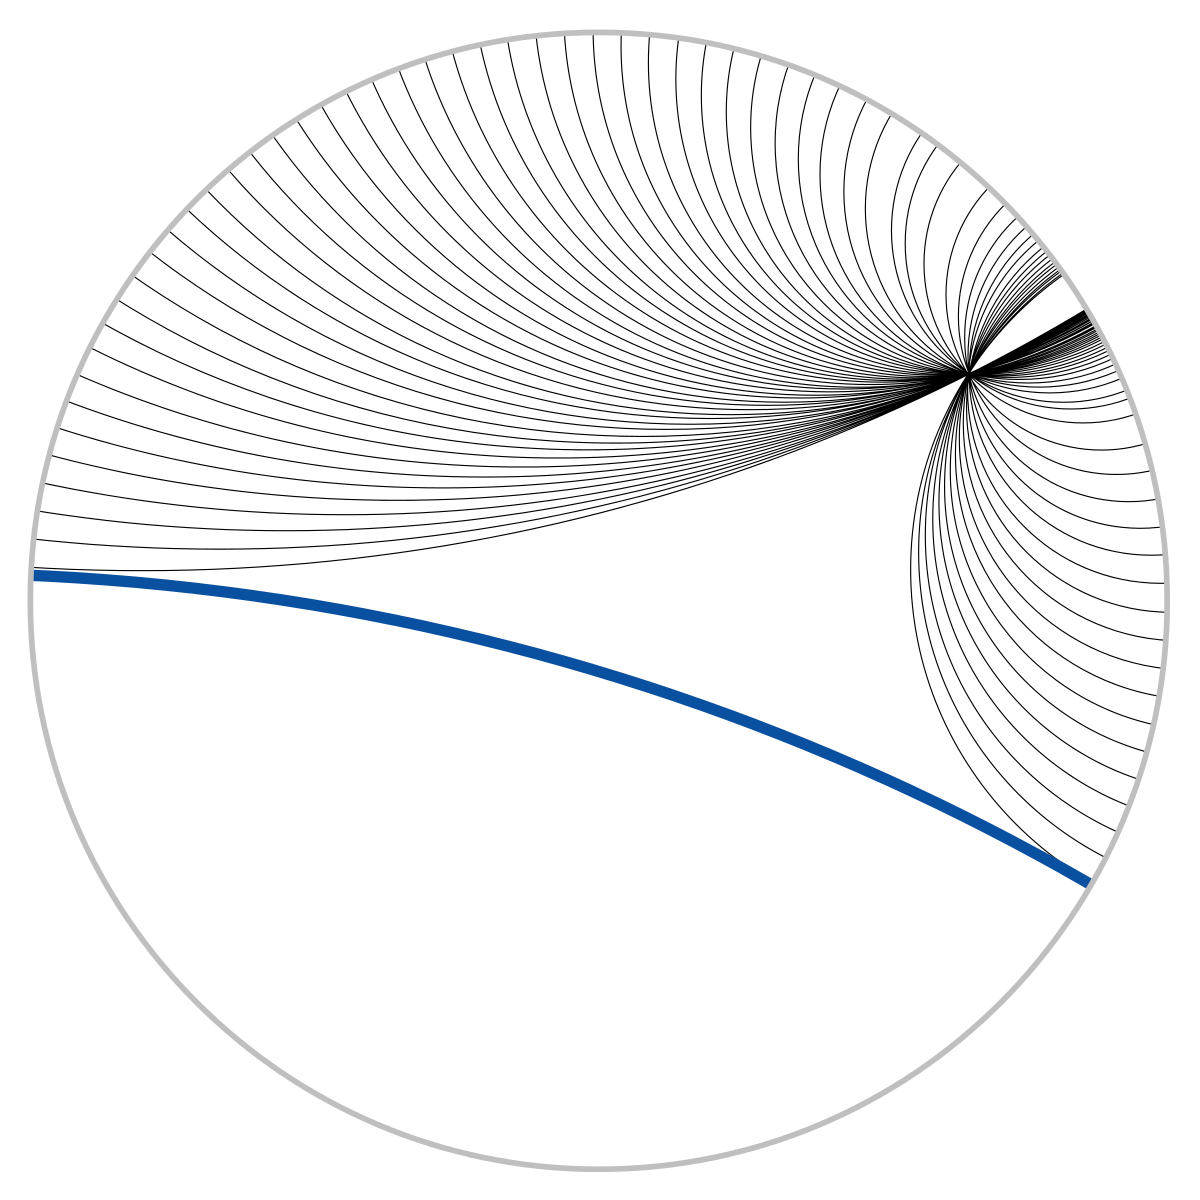
\includegraphics[scale=0.13]{poincare-disk-5aksiom.png}
\caption{Na Poincar\'ejevem disku za dani točko in premico obstaja neskončno vzporednic premici skozi izbrano točko.~\cite[vir slike]{hypGeom-wiki}.}
\end{center}
\end{figure}
%
\end{primer}

%%%%%%%%%%%%%%%%%%%%%%%%%%%%%%%%%%%%%%%%%%%%%%%%%%%%%%%%%%%%%%%%%%%%%%%%%%%%
% Slovar strokovnih izrazov
\section*{Slovar strokovnih izrazov}

\geslo{conformal}{konformen}

\geslo{curvature}{ukrivljenost}

\geslo{geodesic}{geodetka}

\geslo{homogeneous}{homogen}

\geslo{hyperbolic metric}{hiperbolična metrika}

\geslo{hyperbolic space}{hiperboličen prostor}

\geslo{isometry}{izometrija}

\geslo{maximally symmetric/frame homogeneous}{maksimalno simetričen}

\geslo{Riemannian manifold}{Riemannova mnogoterost}

%%%%%%%%%%%%%%%%%%%%%%%%%%%%%%%%%%%%%%%%%%%%%%%%%%%%%%%%%%%%%%%%%%%%%%%%%%%%
% Literatura

\begin{thebibliography}{99}

\bibitem{leeRM} J.~M.~Lee, \emph{Introduction to Riemannian Manifolds}, 2nd ed., Springer International Publishing AG, 2018.

\bibitem{leeSM} J.~M.~Lee, \emph{Introduction to Smooth Manifolds}, 2nd ed., Springer, New York, 2013.

\bibitem{cannon et.} J.~W.~Cannon in drugi, \emph{Hyperbolic Geometry}, Flavours of Geometry, MSRI Publication, \textbf{31}, 1997; dostopno tudi na \url{http://library.msri.org/books/Book31/files/cannon.pdf}.

\bibitem{zapiski} Zapiski s predavanj prof.~B.~Lavriča pri predmetu Elementarna geometrija, Univerza v Ljubljani, Fakulteta za matematiko in fiziko (študijsko leto 2018/2019).

\bibitem{parkkonen} J.~Parkkonen, \emph{Hyperbolic geometry}, [ogled 13.~6.~2021], dostopno na \url{http://users.jyu.fi/~parkkone/RG2012/HypGeom.pdf}.

\bibitem{hypGeom-wiki} Sodelavci Wikipedie, \emph{Hyperbolic geometry}, verzija 10.~6.~2021, [ogled 13.~6.~2021], dostopno na \url{https://en.wikipedia.org/wiki/Hyperbolic_geometry}.

\end{thebibliography}

\end{document}